\section{Vectors in $\R^n$}

\begin{outcome}

\begin{enumerate}
\item[A.] Understand the geometric and algebraic meaning of points and
  vectors in $\R^n$.
\item[B.] Find the position vector of a point in $\R^n$.
\item[C.] Determine whether two vectors are equal.
\end{enumerate}
\end{outcome}

In this section, we define points and vectors in $n$-dimensional
space, and discuss some of their interpretations. We start with a
brief review of Cartesian coordinate systems.
\bigskip

\noindent\textbf{Points in $n$-dimensional space.}
You are probably already familiar with Cartesian
coordinates\index{Cartesian coordinates}, which let you describe
points\index{point} in $2$- or $3$-dimensional space. Consider the
familiar coordinate plane, with an $x$-axis and a $y$-axis. Any point
within this coordinate plane is identified by its $x$- and
$y$-coordinates\index{coordinate of a point}. For example, the point
$P$ in the following diagram has $x$-coordinate~$2$ and
$y$-coordinate~$1$.  We write these coordinates as an ordered pair
$P=(2,1)$. Here, ``ordered'' means that the $x$-coordinate comes
first, and then the $y$-coordinate, i.e., $(1,2)$ is not the same
point as $(2,1)$. Coordinates can be positive, negative, or zero. The
special point with coordinates $(0,0)$ is called the
\textbf{origin}\index{origin} of the coordinate system.
\begin{center}
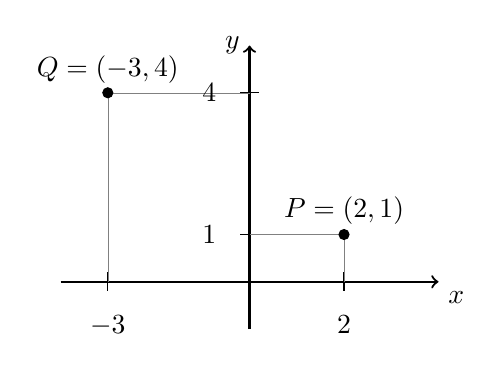
\begin{tikzpicture}[scale=0.6]
\draw[thick,->](-4,0)--(4,0);
\draw[thick,->](0,-1)--(0,5);
\draw(2,0.2)--(2,-0.2);
\draw(-3,0.2)--(-3,-0.2);
\draw(-0.2,1)--(0.2,1);
\draw(-0.2,4)--(0.2,4);
\draw[help lines] (-3,0)--(-3,4)--(0,4);
\draw[help lines](0,1)--(2,1)--(2,0);
\draw[fill](-3,4) circle [radius=3pt];
\draw[fill](2,1) circle [radius=3pt];
\node[below right] at (4,0){$x$};
\node[left] at(0,5){$y$};
\node[below] at (-3,-0.5){$-3$};
\node[below] at (2,-0.5){$2$};
\node[left] at (-0.5, 1){$1$};
\node[left] at (-0.5, 4){$4$};
\node[above] at (-3,4){$Q = (-3,4)$};
\node[above] at (2,1){$P = (2,1)$};
\end{tikzpicture}
\end{center}
The situation in $3$ dimensions is analogous. Here, the coordinate
system has three axes, and each point is described by a triple of
coordinates, which we can write as $(x,y,z)$.  We can extend these
ideas beyond $n=3$. A coordinate system for $n$-dimensional space has
$n$ axes, which we may call $x_1,\ldots,x_n$ (as there are not enough
letters in the alphabet to continue after $z$). A point of
$n$-dimensional space is described by an ordered $n$-tuple
$(x_1,\ldots,x_n)$ of coordinates. For example, $P=(2,1,0,-1)$ is a
point in $4$-dimensional space which has $x_1$-coordinate $2$,
$x_2$-coordinate $1$, and so on. While most people cannot really
picture space beyond $3$ dimensions, it is easy to imagine tuples of
$n$ real numbers. Thus, although we may not be able to ``see'' the
points in higher dimensions, we can still talk about their coordinates.
\bigskip

\noindent\textbf{Vectors in $n$-dimensional space.}
Unlike a point, which describes a location in a coordinate system, a
vector\index{vector!geometrically} describes an {\em
  offset}\index{offset} or a {\em distance and direction}. We usually
picture a vector as an arrow, starting at one point (called the
\textbf{tail}\index{tail} of the arrow) and ending at another point
(called the \textbf{tip}\index{tip} of the arrow).
\begin{center}
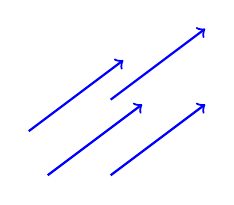
\begin{tikzpicture}[scale=0.8]
\draw[->, thick, blue](1,0)--+(1.5,1.125);
\draw[->, thick, blue](2,1.2)--+(1.5,1.125);
\draw[->, thick, blue](2,0)--+(1.5,1.125);
\draw[->, thick, blue](0.7,0.7)--+(1.5,1.125);
\end{tikzpicture}
\end{center}
Two vectors are considered equal if they have the same direction and
length. Thus, all four blue arrows in the above image describe exactly
the same vector. Mathematically, a vector in $2$-dimensional space is
described as an offset in the $x$-direction and an offset in the
$y$-direction.  For example, a certain vector $\vect{v}$ may be
described by the instruction: ``move $4$ units in the direction
parallel to the $x$-axis, and move $3$ units in the direction parallel
to the $y$-axis''. This situation is pictured here:
\begin{center}
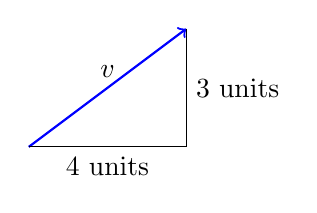
\begin{tikzpicture}[scale=0.5]
  \draw[->, thick, blue](0,0) -- node[above,black]{$\vect{v}$} +(4,3);
  \draw(0,0) -- node[below]{4 units} (4,0) -- node[right]{3 units} (4,3);
\end{tikzpicture}
\end{center}
The numbers $4$ and $3$ are also called the
$x$-component\index{component of a vector} and the $y$-component of
the vector. Notice that a point has ``coordinates'', but a vector has
``components''. We write the components of a vector as an ordered
column within square brackets:
$\vect{v}=\begin{mysmallmatrix}{c}\scriptstyle4\\\scriptstyle3\end{mysmallmatrix}$. Note
that components can also be negative; for example, a negative
$x$-component indicates to move left instead of right, and a negative
$y$-component indicates to move down instead of up. The vector with
all components equal to $0$ is called the \textbf{zero
  vector}\index{zero vector}, and is written $\vect{0}$. 

The situation in $3$ dimensions is similar. Here, a vector is
described by three components, namely, its $x$-component,
$y$-component, and $z$-component. The three components are written as
$\begin{mysmallmatrix}{c}\scriptstyle x\\\scriptstyle y\\\scriptstyle
  z\end{mysmallmatrix}$. The same idea generalizes to $n$-dimensional
vectors when $n$ is greater than $3$. 

\begin{definition}{Column vectors and $\R^n$}{columnvector}
  A $n$-dimensional
  \textbf{column vector}\index{column vector}\index{vector, column},
  often simply called a \textbf{vector}\index{vector}, is an ordered list
  of $n$ real numbers, written as a column within square brackets:
  \begin{equation*}
    \begin{mymatrix}{c}
      x_1 \\
      x_2 \\
      \vdots \\
      x_n
    \end{mymatrix}.
  \end{equation*}
  We write $\R^n$\index{Rn@$\R^n$} for the set of all $n$-dimensional
  column vectors.
\end{definition}
Vectors are usually denoted by boldface lower-case letters such as
$\vect{v}$, $\vect{w}$, $\vect{a}$, $\vect{b}$. Some people write a
small arrow above the vector, but we do not do this here.
\bigskip

\noindent\textbf{Points vs. vectors.}
What is the relationship between points and vectors? Algebraically,
they seem to be almost the same thing, because a point $(x,y)$ and a
vector
$\begin{mysmallmatrix}{c}\scriptstyle x\\\scriptstyle
  y\end{mysmallmatrix}$ are both an ordered pair of real numbers,
written in a slightly different way. On the other hand, geometrically,
a point is a location in space, and has neither a length nor
direction, whereas a vector has length and direction, but is not fixed
at any particular location. Indeed, to convince yourself that despite
the similarity in their notation, points and vectors are different
kinds of objects, imagine that we moved the origin of the coordinate
system to a different location. Then the coordinates of all the points
would change, whereas the components of all the vectors would remain
the same. To describe the components of a vector, we require axes and
a scale, but no origin. To describe the components of a point, we
require axes, a scale, and an origin.  \bigskip

\noindent\textbf{Vectors from points.}
If $Q$ and $P$ are two points in $n$-dimensional space, we can define
a \textbf{vector from $Q$ to $P$}\index{vector!from a point to a point}. This
vector is written $\longvect{QP}$, and is described by the arrow whose
tail is at $Q$ and whose tip is at $P$, as in the following picture:
\begin{center}
  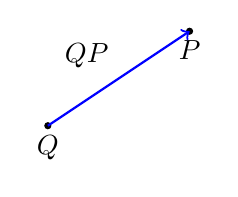
\begin{tikzpicture}[scale=0.6]
    \draw[fill] (0,0) circle [radius=1.8pt] node[below]{$Q$};
    \draw[fill] (3,2) circle [radius=1.8pt] node[below]{$P$};
    \draw[thick, blue, ->](0,0) -- node[above left,black]{$\longvect{QP}$} (3,2);
  \end{tikzpicture}
\end{center}
If the point $Q$ has coordinates $(q_1,\ldots,q_n)$ and the point $P$
has coordinates $(p_1,\ldots,p_n)$, then the components of
$\longvect{QP}$ are
\begin{equation*}
  \longvect{QP} =
  \begin{mymatrix}{c}
    p_1 - q_1 \\
    \vdots    \\
    p_n - q_n
  \end{mymatrix}.
\end{equation*}
An important special case of this is the case when the point $Q$ is
the origin. The following definition is concerned with that situation.

\begin{definition}{The position vector of a point}{positionvector}
  Let $P$ be a point in $n$-dimensional space. The \textbf{position
    vector}\index{position vector} of $P$ is the vector
  $\vect{p} = \longvect{0P}$ whose tail is at the origin and whose tip
  is at $P$.
  \begin{center}
    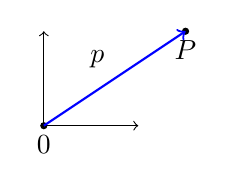
\begin{tikzpicture}[scale=0.6]
      \draw[<->](2,0,0)--(0,0,0)--(0,2,0);
    \draw[fill] (0,0) circle [radius=1.8pt] node[below]{$0$};
    \draw[fill] (3,2) circle [radius=1.8pt] node[below]{$P$};
    \draw[thick, blue, ->](0,0) -- node[above left,black]{$\vect{p}$} (3,2);
    \end{tikzpicture}
  \end{center}
  If the point $P$ has coordinates $(p_1,\ldots,p_n)$, then the
  components of the position vector are
  \begin{equation*}
    \vect{p} =
    \begin{mymatrix}{c}
      p_1    \\
      \vdots \\
      p_n
    \end{mymatrix}.
  \end{equation*}
  Thus, the coordinates of a point are the same as the components of
  its position vector. For this reason, the position vector is also
  sometimes called the
  \textbf{coordinate vector}\index{coordinate vector} of $P$.
\end{definition}

\noindent\textbf{Points from vectors.} Conversely, given any vector
$\vect{p}$, we may find a point $P$ that has $\vect{p}$ as its
position vector. To do so geometrically, we first have the move the
vector $\vect{p}$ around until its tail is at the origin. The point
$P$ will then be located at its tip.
\begin{center}
  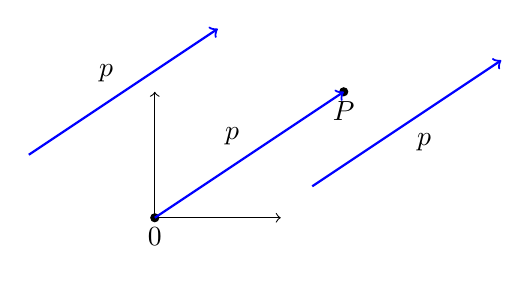
\begin{tikzpicture}[scale=0.8]
    \draw[<->](2,0,0)--(0,0,0)--(0,2,0);
    \draw[fill] (0,0) circle [radius=1.8pt] node[below]{$0$};
    \draw[fill] (3,2) circle [radius=1.8pt] node[below]{$P$};
    \draw[thick, blue, ->](-2,1) -- node[above left,black]{$\vect{p}$} +(3,2);
    \draw[thick, blue, ->](2.5,0.5) -- node[below right,black]{$\vect{p}$} +(3,2);
    \draw[thick, blue, ->](0,0) -- node[above left,black]{$\vect{p}$} +(3,2);
  \end{tikzpicture}
\end{center}
Algebraically, if the vector $\vect{p}$ has components
\begin{equation*}
  \vect{p} =
  \begin{mymatrix}{c}
    p_1    \\
    \vdots \\
    p_n
  \end{mymatrix},
\end{equation*}
then the point $P$ will have coordinates $(p_1,\ldots,p_n)$. This is
just the opposite process of Definition~\ref{def:positionvector}.

So although we went to some lengths to point out that vectors and
points are different geometric objects, as soon as an origin of a
coordinate system has been fixed, we can always talk about a point by
talking about its coordinate vector. We will systematically do so, and
eventually the distinction between a point and its coordinate vector
will become blurred, so that we will be able to talk about $\R^n$ as
``a set of points'' or ``a set of vectors'' interchangeably.  \bigskip

\noindent\textbf{Equality of vectors.}
Two vectors are equal precisely when all corresponding components are
equal. In symbols, if
\begin{equation*}
  \vect{u} =
  \begin{mymatrix}{c}
    u_1\\
    \vdots\\
    u_n
  \end{mymatrix}
  \quad\mbox{and}\quad
  \vect{v} =
  \begin{mymatrix}{c}
    v_1\\
    \vdots\\
    v_n
  \end{mymatrix},
\end{equation*}
then $\vect{u}=\vect{v}$ if and only if $u_1=v_1$ and $u_2=v_2$ and
\ldots and $u_n=v_n$.
\bigskip

\noindent\textbf{Notation.}
In the text, it is often awkward to write column vectors, because they
take up so much space. To save space, we sometimes use a superscript
``$T$'' to denote a column vector. For example, we write
$\begin{mymatrix}{rrr}1&2&3\end{mymatrix}^T$, or sometimes
$\mat{1, 2, 3}^T$, to denote the vector
\begin{equation*}
  \begin{mymatrix}{c}
    1\\
    2\\
    3\\
  \end{mymatrix}.
\end{equation*}
The letter ``$T$'' stands for ``transpose''. To transpose a vector
means to turn a row into a column or vice versa.

% ----------------------------------------------------------------------

